\chapter{CloneRefactor} \label{ch:clonerefactor}
% We bridged a gap between clone detection and refactoring .. by designing a tool
CloneRefactor is the name of our clone detection and refactoring tool. It features the following novel functions:
\begin{itemize}
  \item Detection of clone classes rather than clone pairs.
  \item A novel detection method, aimed at extensibility.
  \item Detection of refactoring-oriented clone types, in addition to the literature clone types.
  \item Allows for automated refactoring of a subset of the detected duplication issues.
\end{itemize}
In this section we describe our approach and rationale for the design decisions regarding this tool.

\begin{figure}[H]
  \centering
  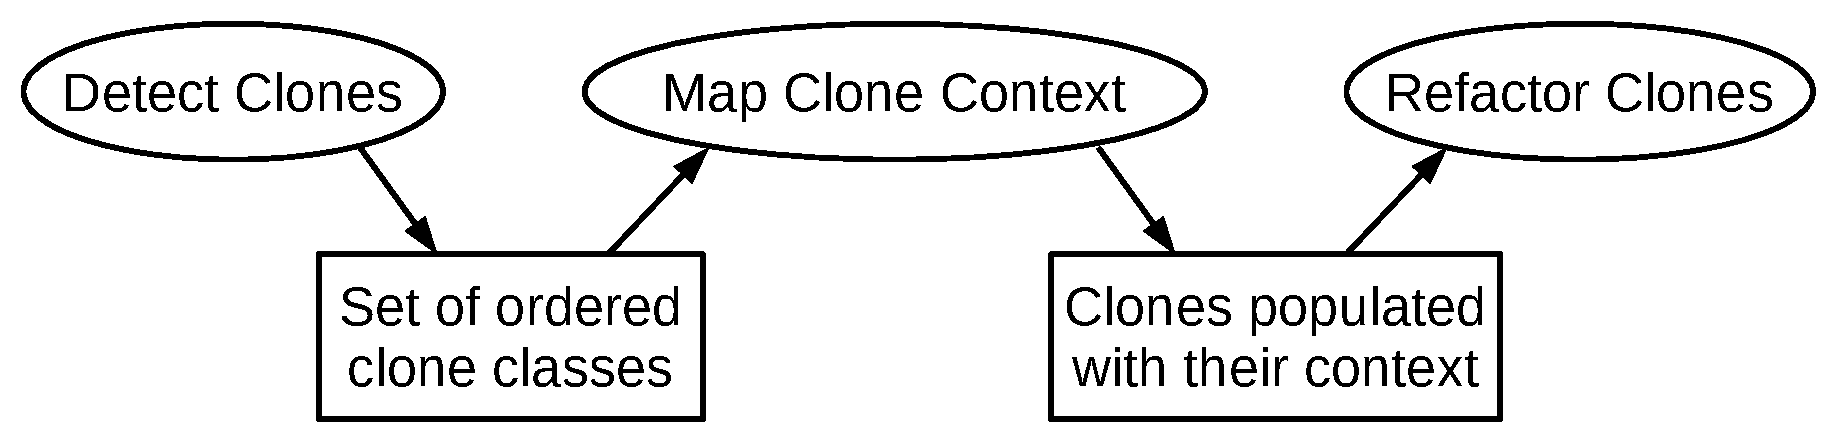
\includegraphics[width=0.8\columnwidth]{img/CloneRefactorOverall}
  \caption{CloneRefactor overall process.}
  \label{fig:clonerefactorprocess}
\end{figure}

Figure \ref{fig:clonerefactorprocess} shows the overall process used by CloneRefactor. First, we detect clones on basis of a Java codebase, given a Java project from disk and a configuration. The clone detection process is further explained in section \ref{sec:clonedetection}. After all clones are found, CloneRefactor maps the context of the clones. On basis of this context, CloneRefactor applies transformations to the source code for clones for which we have configured a refactoring.

\section{JavaParser}
A very important design decision for CloneRefactor is the usage of a library named JavaParser \cite{tomassetti2017javaparser}. JavaParser is a Java library which allows to parse Java source files to an abstract syntax tree (AST\footnote{An AST is a tree-representation of a source code file.}). JavaParser allows to modify this AST and write the result back to Java source code. This allows us to apply refactorings to the detected problems in the source code.

Integrated in JavaParser is a library named SymbolSolver. This library allows for the resolution of symbols using JavaParser. For instance, we can use it to trace references (methods, variables, types, etc) to their declarations (these referenced identifiers are also called ``symbols''). This is very useful for the detection of our refactoring-oriented clone types, as they make use of the fully qualified identifiers of symbols.

In order to be able to trace referenced identifiers SymbolSolver requires access to not only the analyzed Java projects, but also all its dependencies. This requires us to include all dependencies with the project. Along with this, SymbolSolver solves symbols in the JRE System Library (the standard libraries coming with every installation of Java) using the active Java Virtual Machine (JVM). This has a big impact on performance efficiency.

Because of the requirement of symbol resolution, the refactoring-oriented clone types are less suitable for large scale clone analysis.

\section{Thresholds}\label{sec:clonerefactorthresholds}
CloneRefactor operates on a set of thresholds to determine the validity of clones that are found. In general, these thresholds are:
\begin{itemize}
  \item \textbf{Minimum Amount of Nodes}: The minimum amount of nodes that should be in each instance of cloned fragements for them to be considered a clone class.
  \item \textbf{Minimum Amount of Tokens}: The minimum amount of tokens that should be in each instance of cloned fragements for them to be considered a clone class.
  \item \textbf{Minimum Amount of Lines}: The minimum amount of lines that should be in each instance of cloned fragements for them to be considered a clone class.
\end{itemize}

When we analyze type 2R or type 3R clones we use the following additional threshold:
\begin{itemize}
  \item \textbf{T2R Variability}: The percentage of variability we allow in variables, method calls and literals. How this threshold is calculated is explained in section \ref{sec:t2rcheckglobalthres}.
\end{itemize}

When we analyze type 3 or type 3R clones we use the following additional threshold:
\begin{itemize}
  \item \textbf{T3R Gap Size}: The size of the gap we allow between two valid clones. This is a percentage of the size of the gap against the size of both clones combined. How this threshold is calculated is further explained in section \ref{sec:t3rclonerefactor}.
\end{itemize}

\section{Clone Detection}\label{sec:clonedetection}
To detect clones, CloneRefactor parses the AST aqcuired from JavaParser to an unweighted graph structure. On basis of this graph structure, clones are detection. Dependent on the type of clones being detected, transformations may be applied. The way in which CloneRefactor was designed does not allow for several clone types to be detected simultaneously, in accordance with our clone type philosophy as described in chapter \ref{sec:unifying}.

The overall process regarding clone detection is displayed in figure \ref{fig:clonedetection}. First of all, we use JavaParser to read a project from disk and build an AST, one class file at a time. Each AST is then converted to a directed graph that maps relations between statements, further explained in section \ref{sec:clonegraph}. On basis of this graph, we detect clone classes and verify them using three thresholds (in order of importance):
\begin{itemize}
  \item Amount of tokens.
  \item Amount of statements.
  \item Amount of lines.
\end{itemize}
If the detection was configured to detect either type 2R, 3 or 3R clones we perform some type specific transformations on the resulting set of clones.

\begin{figure}[H]
  \centering
  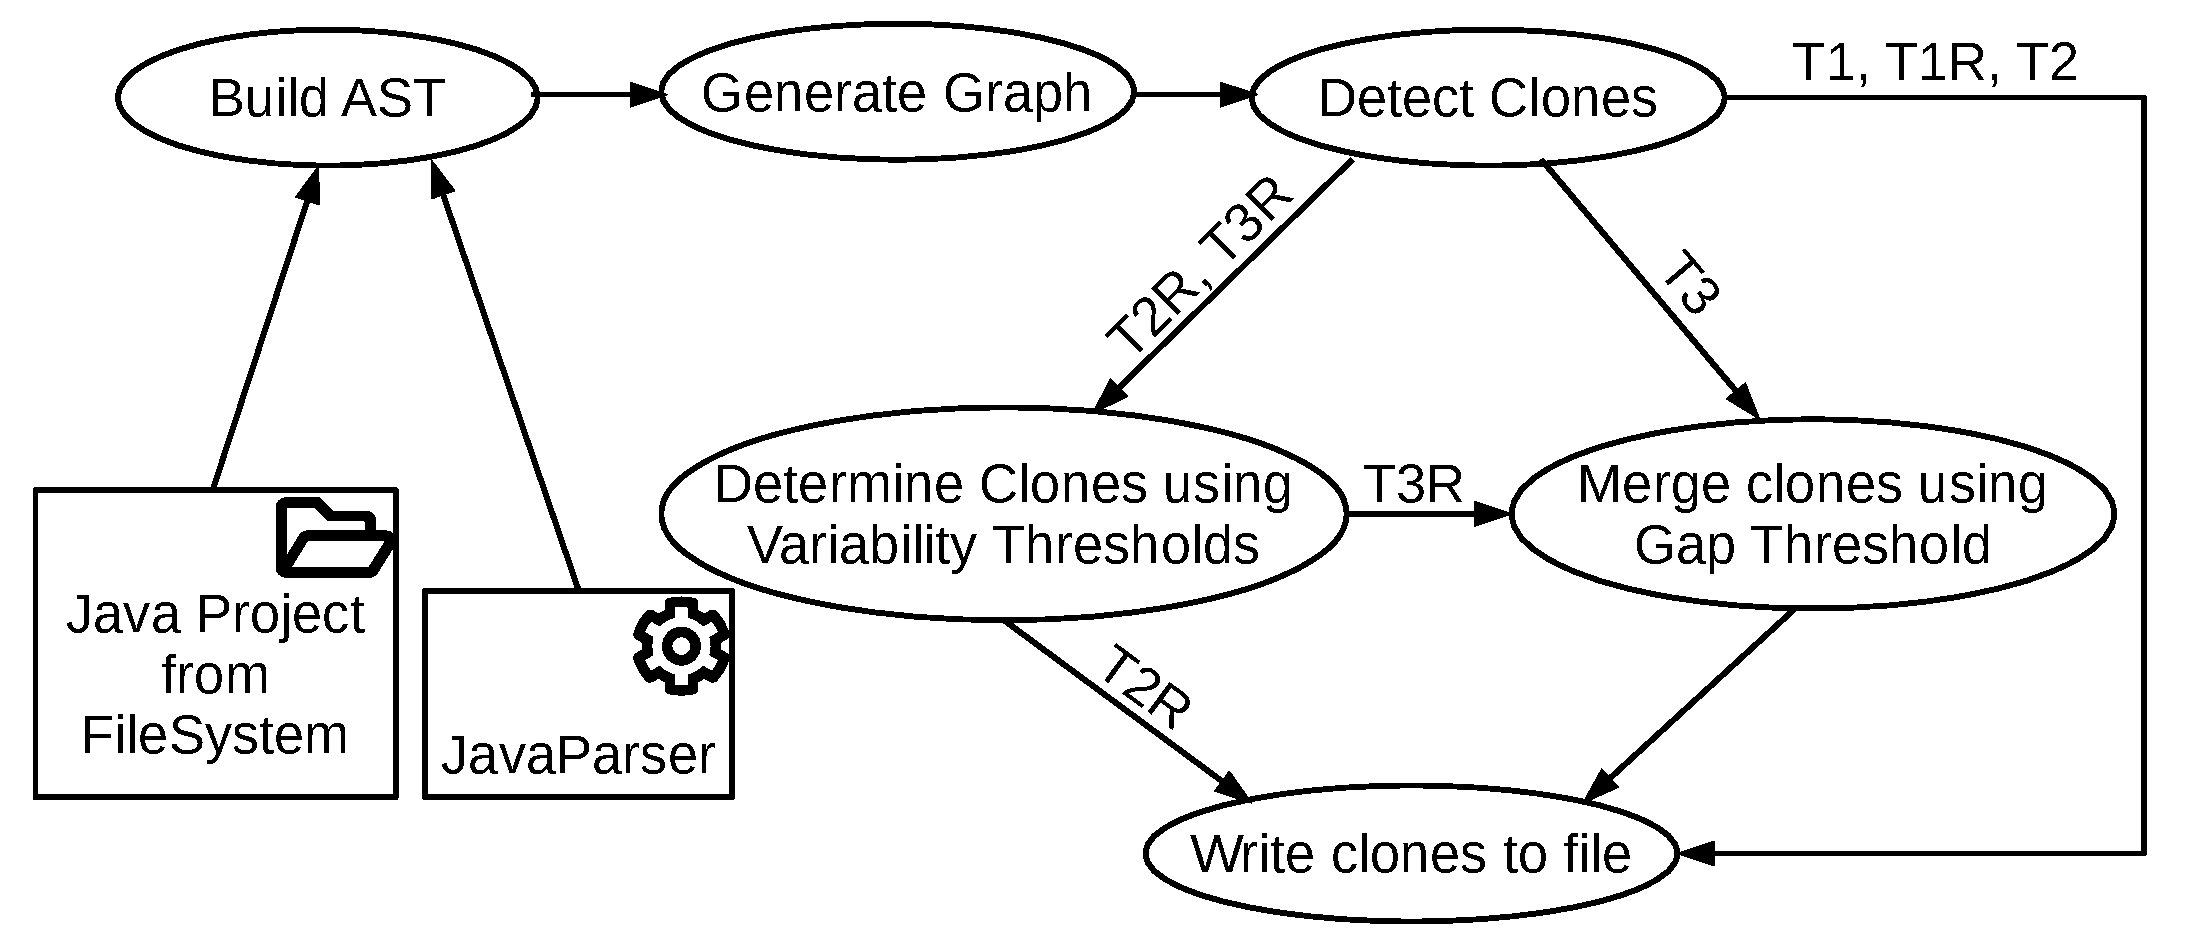
\includegraphics[width=1\columnwidth]{img/CloneDetection}
  \caption{CloneRefactor clone detection process.}
  \label{fig:clonedetection}
\end{figure}

\subsection{Generating the clone graph}\label{sec:clonegraph}
First of all, we parse the AST obtained from JavaParser into a directed graph structure. We have chosen to base our clone detection around statements as the smallest unit of comparison. This means that a single statement cloned with another single statement is the smallest clone we can find. The rationale for this lies in both simplicity and performance efficiency. This means we won't be able to find when a single expression matches another expression, or even a single token matching another token. This is in most cases not a problem, as expressions are often small and do not span the minimal size to be considered a clone in the first place (more about this in section \ref{sec:thresholds}).

\subsubsection{Filtering the AST}
As a first step towards building the clone graph, we preprocess the AST to decide which AST nodes should become part of the clone graph. We have decided to consider declarations and statements as the smallest compared entities. The main reasoning for this is because considering smaller AST constructs, like expressions, significantly increases the complexity and CPU usage of our clone detection and refactoring efforts.

Additionally, we exclude package declarations and import statements. These are omitted by most clone detection tools, as clones in import statements hold limited valuable information.

\subsubsection{Building the clone graph}\label{sec:buildingclonegraph}
Building the clone graph consists of walking the AST in-order for each declaration and statement. For each declaration/statement found, we map the following relations:
\begin{itemize}
  \item The declaration/statement preceding it.
  \item The declaration/statement following.
  \item The last \textbf{preceding} declaration/statement with which it is cloned.
\end{itemize}
We do not create a separate graph for each class file, so the statement/declaration preceding or following could be in a different file. While mapping these relations, we maintain a hashed map containing the last occurrence of each unique statement. This map is used to efficiently find out whether a statement is cloned with another. An example of such a graph is displayed in figure \ref{fig:clonegraphsimple}.

\begin{figure}[H]
  \centering
  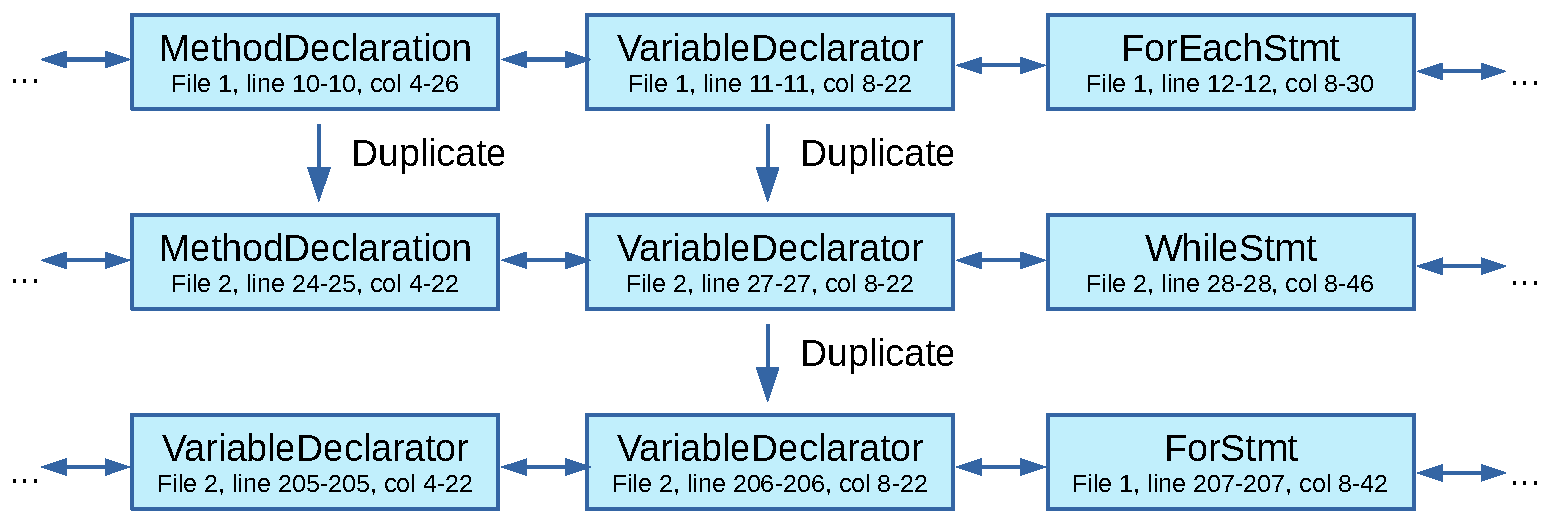
\includegraphics[width=1\columnwidth]{img/CodeGraph2}
  \caption{Abstract example of a part of a possible clone graph as built by CloneRefactor.}
  \label{fig:clonegraphsimple}
\end{figure}

We refer to the declarations and statements in this graph as \textit{nodes}. The relations \textit{next} and \textit{previous} in this graph are represented as an twodirectional arrow. The relations representing duplication are directed. This is a restriction we've chosen as it creates an important constraint for the clone detection process. This process is explained in section \ref{sec:detectingclones}.

\subsubsection{Comparing Statements/Declarations} \label{sec:comparingstuff}
In the previous section we described a ``duplicate'' relation between nodes in the clone graph built by CloneRefactor. Whether two nodes in this graph are duplicates of each other is dependent on the clone type. In this section, we will describe for each type how we compare statements and declarations to assess whether they are clones of each other.

CloneRefactor detects six different types of clones: T1, T2, T3, T1R, T2R and T3R. These types are further explained in chapter \ref{chap:clonetypes}. For \textbf{type 1} clones, CloneRefactor filters the tokens of a node to exclude its comments, whitespace and end of line (EOL) characters and then compares these tokens. For \textbf{type 2} clones, the tokens are further filtered to omit all identifiers and literals. \textbf{Type 3} clones do the same duplication comparison as type 2 clones.

For \textbf{type 1R} clones, this comparison is a lot more advanced. For \textit{method calls} we trace their declaration and use its fully qualified method signature for comparison with other nodes. For all \textit{referenced types} we trace their declarations and use assemble their fully qualified identifier for comparison with other nodes. For \textit{variables} we trace their declaration and their types. If the variable type is a primitive we can directly use it for comparison. If it is a referenced type, we have to trace this type first in order to collect their fully qualified identifier for comparison.

\textbf{Type 2R} clones allow any variation in literals, variables and method calls at this stage in the clone detection process. However, for \textit{literals} we do resolve their type in order to verify that they are of the same type. For \textit{variables} we also only verify that their types are the same (but not their names). For \textit{method calls}, we trace their declaration but only compare the fully qualified identifier for its return type and each of its arguments' types. Apart from that, we do not compare the names of method, class, interface and enum declarations.

In this stage, \textbf{type 3R} clones have the same compare rules as type 2R clones.

\subsubsection{Mapping graph nodes to code}
The clone graph, as explained in section \ref{sec:buildingclonegraph}, contains all declarations and statements in a source code. However, declarations and statements may themselves have child declarations and statements. To avoid redundant duplication checks, we exclude child declarations and statements from each node. Look at figure \ref{fig:clonegraph} for an example of how source code maps to AST nodes.

\begin{figure}[H]
  \centering
  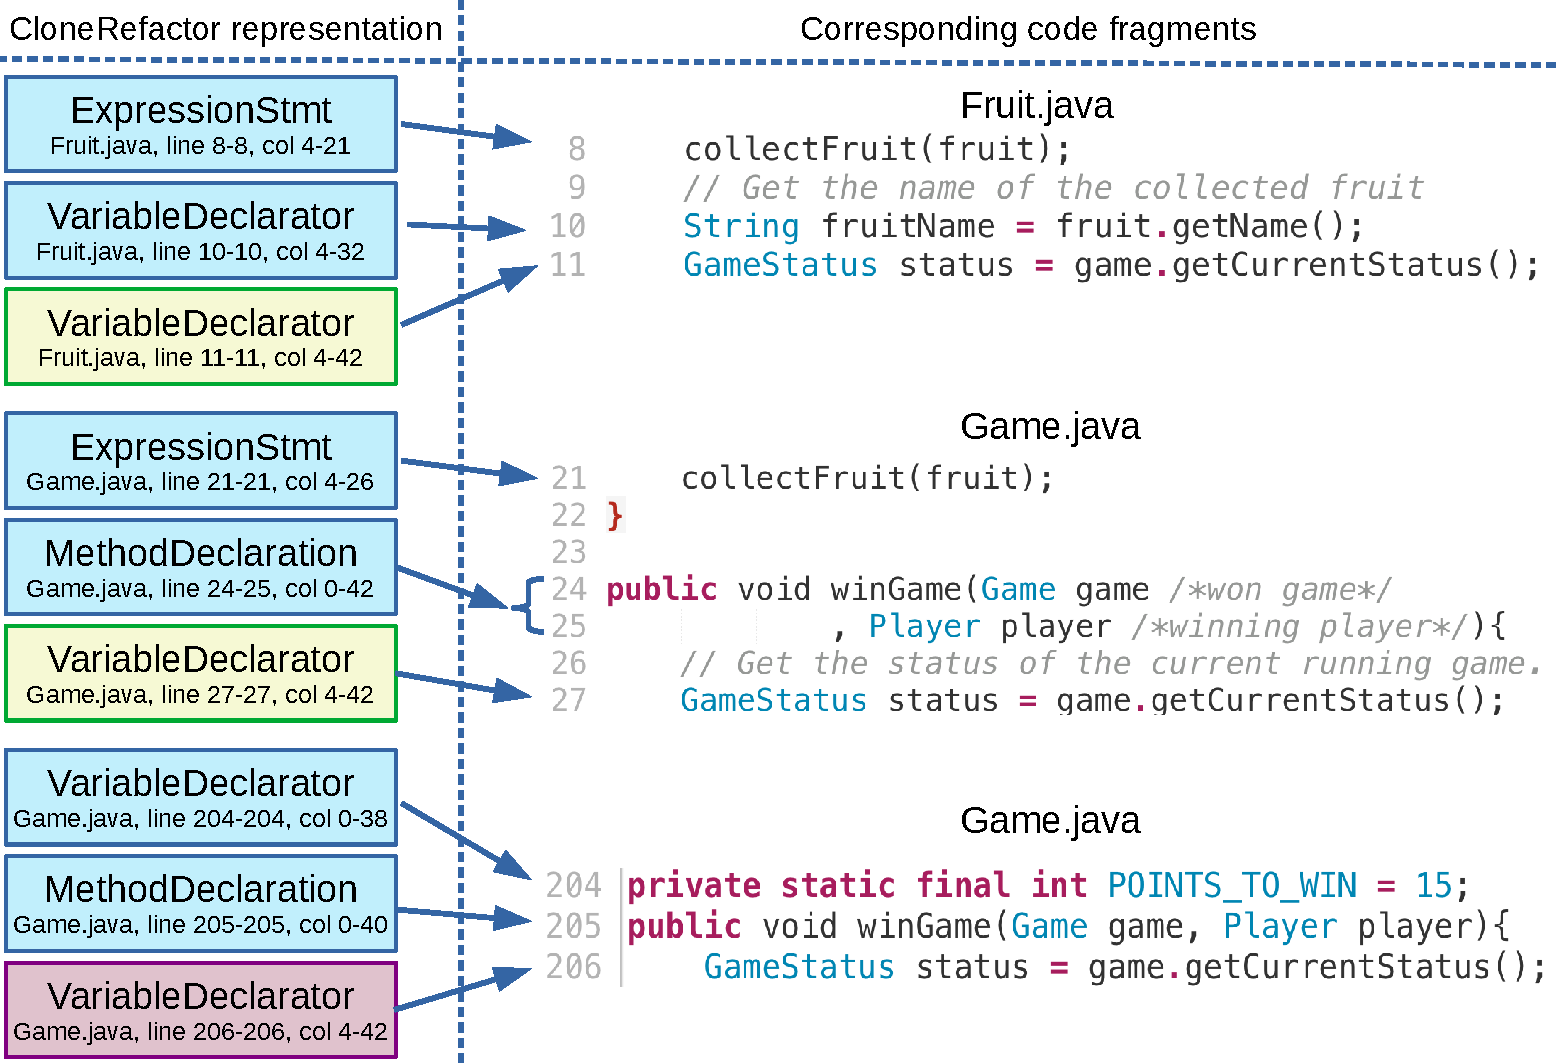
\includegraphics[width=1\columnwidth]{img/CloneGraphCode}
  \caption{CloneRefactor extracts statements and declarations from source code.}
  \label{fig:clonegraph}
\end{figure}

In line 24-25 of the code fragment, we see a \texttt{MethodDeclaration}. The node corresponding with this MethodDeclaration denotes all tokens found on these two lines, line 24 and 25. Although the statements following this method declaration (those that are part of its body) officially belong to the method declaration, they are not included in its graph node. Because of that, in this example, the \texttt{MethodDeclaration} on line 24-25 will be considered a clone of the \texttt{MethodDeclaration} on line 205 even though their bodies might differ. Even the range (the line and column that this node spans) does not include its child statements and declarations.

\subsection{Detecting Clones} \label{sec:detectingclones}
After building the clone clone graph, we use it to detect clones. We decided to focus on the detection of clone classes rather than clone pairs because clone pairs do not provide a general overview of all entities containing the clones, with all their related issues and characteristics \cite{fontana2012duplicated}. Although clone classes are harder to manage, they provide all information needed to plan a suitable refactoring strategy, since this way all instances of a clone are considered. Another issue that results from grouping clones by pairs: clone reference amount increases according to the binomial coefficient formula (two clones form a pair, three clones form three pairs, four clones form six pairs, and so on), which causes a heavy information redundancy \cite{fontana2012duplicated}.

As stated in the previous section, nodes in the graph link to \textit{preceding} cloned statement. This implies that the first node that is cloned does not have any clone relation, as there are no clones preceding it (only following it). Because of this, we start our clone detection process at the final location encountered while building the graph. For this node, we collect all nodes it is cloned with. Even though the final node only links to the preceding node it is cloned with, we can collect all clones. This is because the preceding clone also has a preceding clone (if applicable) and we can follow this trail to collect all clones of a single node. As an example, we convert the code example shown in figure \ref{fig:clonegraph} to a clone graph as displayed in figure \ref{fig:clonegraph2}.

\begin{figure}[H]
  \centering
  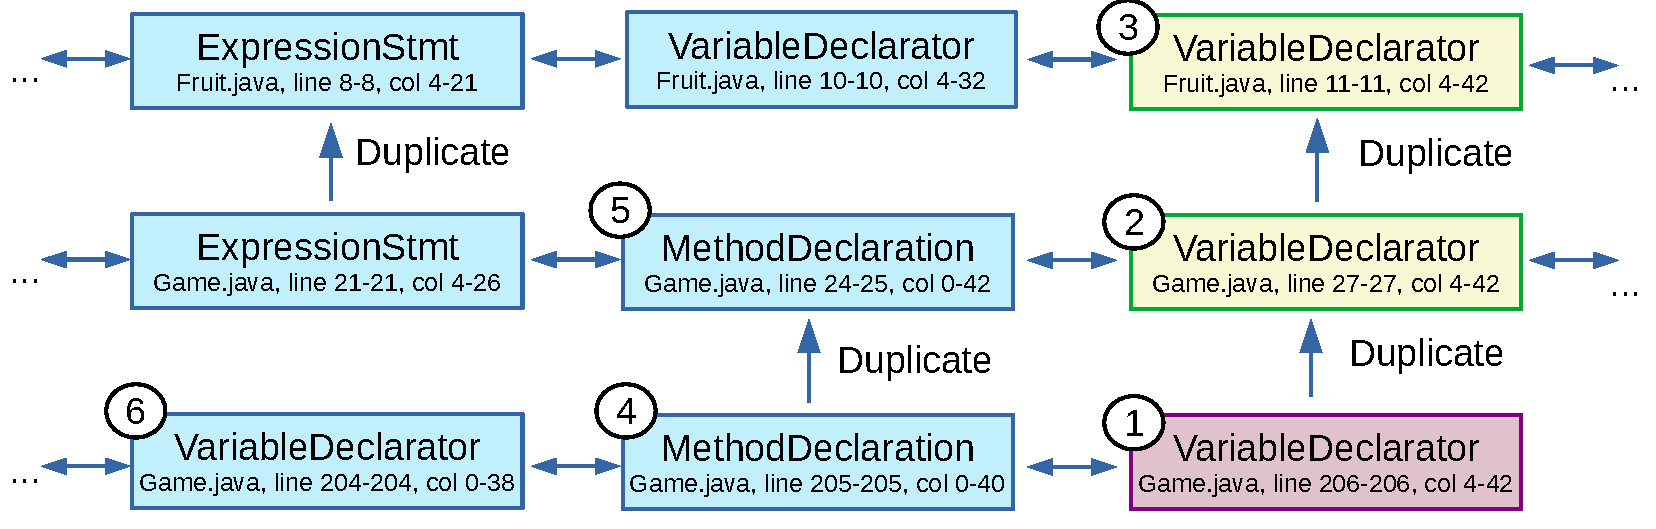
\includegraphics[width=1\columnwidth]{img/CodeGraphExample}
  \caption{Example of a clone graph built by CloneRefactor.}
  \label{fig:clonegraph2}
\end{figure}

Using the example shown in figure \ref{fig:clonegraph} and \ref{fig:clonegraph2} we can explain how we detect clones on basis of this graph. Suppose we are finding clones for two files and the final node of the second file is a variable declarator. This final node is represented in the example figure by the purple box (1). We then follow all ``duplicate'' relations until we have found all clones of this node (2 and 3). We now have a single statement clone class of three clone instances (1, 2 and 3).

Next, we move to the previous line (4). Here again, we collect all duplicates of this node (4 and 5). For each of these duplicates, we check whether the node following it is already in the clone class we collected in the previous iteration. In this case, (2) follows (5) and (1) follows (4). This means that node (3) does not form a `chain' with other cloned statements. Because of this, the clone class of (1, 2 and 3) comes to an end. It will be checked against the thresholds, and if adhering to the thresholds, considered a clone.

We then go further to the previous node (6). In this case, this node does not have any clones. This means we check the (2 and 5, 1 and 4) clone class against the thresholds, and if it adheres, consider it a clone. Dependent on the thresholds, this example can result in a total of two clone classes.

Eventually, following only the ``previous node'' relations, we can get from (6) to (2). When we are at that point, we will find only one cloned node for (2), namely (3). However, after we check this clone against the thresholds, we check whether it is a subset of any exisiting clone. If this is the case (which it is for this example), we discard the clone.

\subsubsection{Removing redundant clone classes}\label{sec:conceptualremovingredundant}
The clone detection method used by CloneRefactor can, for various reasons,%Should I list these? Listing them could be a section on its own, as I'd have to show examples to make it concrete.
result in redundant clone classes. After the insertion of each newly detected clone, we check whether it is redundant and/or any of the existent clones has become redundant by adding this clone. A clone is redundant if it is a subset of another clone. We define the subset relation between clones as follows:

\begin{equation}\label{eq:subset}
C_1 \subseteq C_2 := \forall (i_1 \in C_1) \text{ } \exists (i_2 \in C_2) \text{ } F i_1 = F i_2 \wedge R i_1 \subseteq R i_2
\end{equation} % Right symbol for definition

Where \textit{C} refers to a clone class (a set of clone instances), \textit{i} refers to a clone instance, \textit{F} is the file in which a clone instance is located and \textit{R} is the range of tokens that a clone instance spans. For each clone found, we remove all existing clones that are a subset of the found clone:

\begin{equation}\label{eq:removeall}
S_{after} = S_{before} \setminus \{C_{existing} \subseteq C_{new}\text{ }|\text{ }C_{existing} \in S_{before}\}
\end{equation}

Where \textit{$S_{before}$} is the clone class collection containing all clones that are found up in until this point and \textit{$C_{new}$} is the clone class that was just found. \textit{$S_{after}$} is the clone class collection after

We should not add the new clone to our list of clones if its a subset of an existing clone. Because of that, we check for each clone added whether there exists a clone class of which the found clone class is a subset:

\begin{equation}\label{eq:removeexisting}
\{C_{existing} \subseteq C_{new}\text{ }|\text{ }C_{existing} \in S\} = \emptyset \Rightarrow S_{after} = S \cup C_{new}
\end{equation}

If the newly added clone is a subset of an existing clone, we do not add it to the set of clone classes. This way we avoid redundant clone classes being detected by CloneRefactor.

\subsection{Validating the type 2R variability threshold}
In the definition of type 2R clones (see section \ref{sec:type2r}) we described how type 2R clones work on basis of a variability threshold. This threshold is checked by CloneRefactor to assess the validity of found clone classes. Implementing such a threshold involves some important design decisions and has a lot of underwater complexity. In this section we explain how CloneRefactor detects type 2R clones on basis of this variability threshold. This process is done as a postprocessing step after clone detection. The type 2R clone detection process is described in more detail in section \ref{sec:comparingstuff}. In short, this process detects clones allowing for any variability between expressions. This postprocessing step then determines which (parts of) these clones are valid by the configure variability threshold.

\begin{figure}[H]
  \centering
  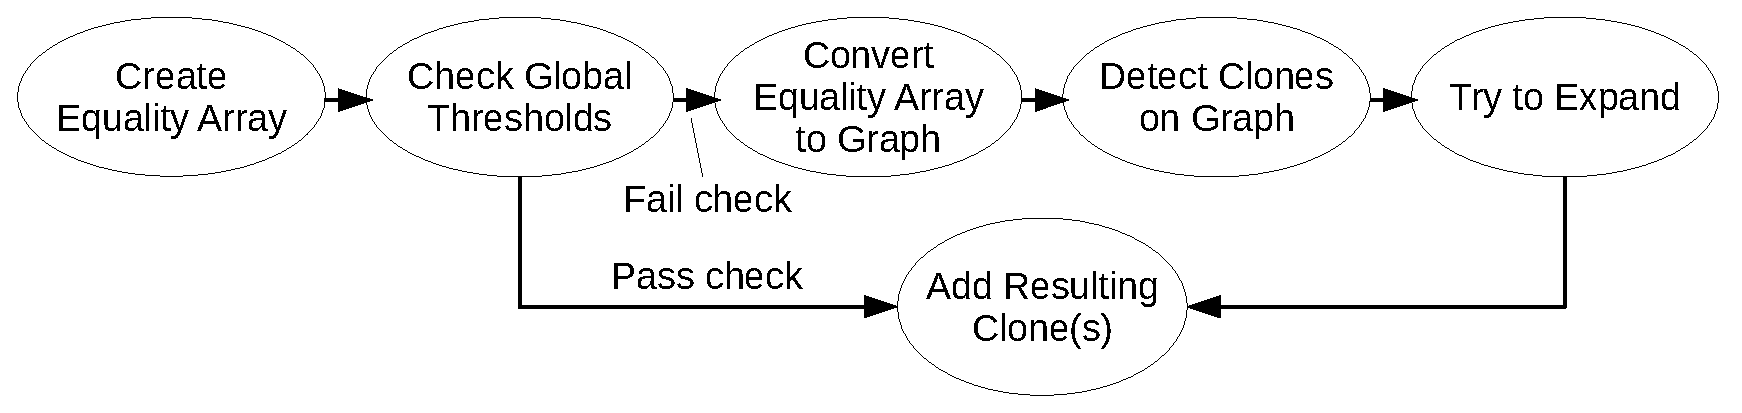
\includegraphics[width=1\columnwidth]{img/CloneRefactorT2RFlow}
  \caption{Process used to check the variability threshold for T2R clones.}
  \label{fig:clonerefactort2rflow}
\end{figure}

Figure \ref{fig:clonerefactort2rflow} shows the steps that CloneRefactor performs to find clones conforming with the type 2R variability threshold. Each of the following paragraphs will explain a step from this figure.

\subsubsection{Create equality array}
To determine the difference in literals, method calls and variables, we convert the code to an equality array. This equality array converts each (group of) token(s) to a number unique to that (group of) tokens. Each literal, method call or variable becomes a positive number, whereas each other token becomes a negative number. An example of two code fragments converted to equality arrays is displayed in figure \ref{fig:equalityarrays}.

\begin{figure}[H]
  \centering
  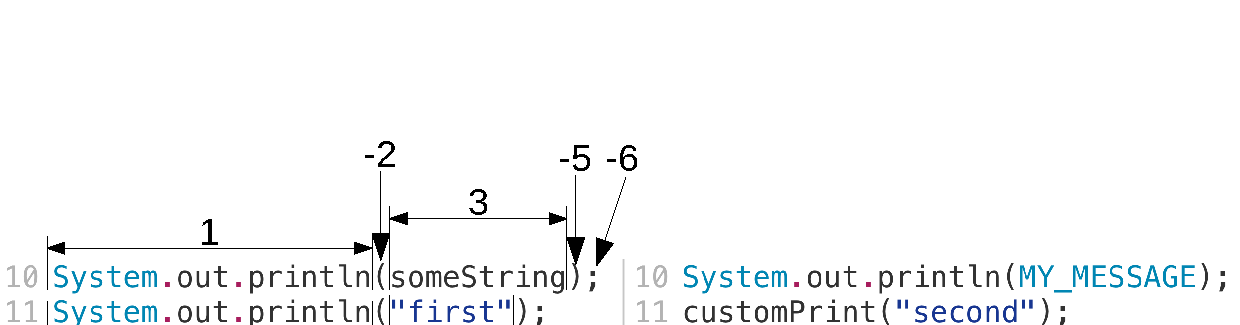
\includegraphics[width=1\columnwidth]{img/equality}
  \caption{The conversion of code to an equality array.}
  \label{fig:equalityarrays}
\end{figure}

The equality array for each of the lines in this example is shown in table \ref{table:equalityarrays}.

\begin{table}[H]
\begin{center}
 \caption{The equality arrays in our example figure \ref{fig:equalityarrays}.} \label{table:equalityarrays}
 \medskip
\begin{tabular}{|l|l|l|}
\hline
Node (n) & Equality Array (E) \\ \hline
1        & {[}1, -2, 3, -5, -6{]} \\ \hline
2        & {[}1, -2, 7, -5, -6{]} \\ \hline
3        & {[}1, -2, 4, -5, -6{]} \\ \hline
4        & {[}8, -2, 9, -5, -6{]} \\ \hline
\end{tabular}
\end{center}
\end{table}

In the example of figure \ref{fig:equalityarrays} the fragment on the left (consisting of $n_1$ and $n_2$) and the fragment on the right (consisting of $n_3$ and $n_4$) are two clone instances of a clone class. Table \ref{table:equalityarrays} shows their corresponding equality arrays.

\subsubsection{Checking global thresholds} \label{sec:t2rcheckglobalthres}
Using the equality arrays explained in the previous section, we can determine the variability threshold of any clone class. We calculate the variability of the example given in table \ref{table:equalityarrays} as follows:

\begin{equation}\label{eq:variabilityclonerefactor}
\text{T2R Variability} = \frac{|\{x>0 \land y>0 \land x \neq y \Rightarrow (x,y) \text{ }|\text{ }x \in E_1 \cup E_2, y \in E_3 \cup E_4\}|}{|\{x>0 \land y>0 \Rightarrow (x,y) \text{ }|\text{ }x \in E_1 \cup E_2, y \in E_3 \cup E_4\}|}*100
\end{equation}

Where $E_x$ refers to the equality arrays shown in table \ref{table:equalityarrays} and \textit{x} is the node number displayed in the same table. When we apply this equation to the example clone classes displayed in figure \ref{fig:equalityarrays}, we get the following sum:

\begin{equation}\label{eq:sumequality}
\frac{|\{(3,4), (1,8), (7,9)\}|}{|\{(1,1), (3,4), (1,8), (7,9)\}|}*100 = \frac{3}{4}*100 = 75\%
\end{equation}

So for the example given in figure \ref{fig:equalityarrays} we have a variability of 75r \%. In CloneRefactor, the maximum variability percentage is a threshold that is entered in a configuration file. If a clone adheres to this threshold, it will stay in the set of found clones. However, if it does not adhere to the thresholds, a problem arises. Because a clone does not adhere to the thresholds, it does not yet mean it has to be discarded. This is because an invalid clone class can still contain valid clones that are a subset of the invalid clone (our definition of subsets of clones is given in section \ref{sec:conceptualremovingredundant}).

%Two nodes are considered clones of each other if the size of their equality array is equal and all negative numbers in the equality array are equal.


When a found clone class does not adhere to the global thresholds as explained in the previous section, we need to determine whether it contains any valid subclones. Below, we explain a few cases of valid subclones that may exist within an invalid clone class.

\begin{figure}[H]
\begin{parcolumns}{2}
\colchunk[1]{
\begin{javacode}
doA(a, b, c);
|\highlightYellow|doA();
|\highlightYellow|doB();
|\highlightYellow|doC();
\end{javacode}}
\colchunk[2]{
\begin{javacode}
doB(d, e, f);
|\highlightYellow|doA();
|\highlightYellow|doB();
|\highlightYellow|doC();
\end{javacode}}
\end{parcolumns}
\caption{One node in a type 2R clone has a high variability.}
\label{fig:2rvariabilityhigh1}
\end{figure}

The first line of the cloned fragment shown in figure \ref{fig:2rvariabilityhigh1} has a high variability with its cloned fragement. However, the rest of this method does not have any variability. The global thresholds could indicate a too high variability and thus render this clone invalid. However, in this case, it might still have a valid subclone.

\begin{figure}[H]
\begin{parcolumns}{3}
\colchunk[1]{
\begin{javacode}
|\highlightYellow|doA();
|\highlightYellow|doB();
|\highlightYellow|doC();
\end{javacode}}
\colchunk[2]{
\begin{javacode}
|\highlightYellow|doA();
|\highlightYellow|doB();
|\highlightYellow|doC();
\end{javacode}}
\colchunk[3]{
\begin{javacode}
doD();
doE();
doF();
\end{javacode}}
\end{parcolumns}
\caption{One clone instance in a type 2R clone has a high variability.}
\label{fig:2rvariabilityhigh2}
\end{figure}

Another example of high variability between clones, in which a valid subclone can be found, is displayed in figure \ref{fig:2rvariabilityhigh2}. In this case, one clone instance has such a high variability that it shouldn't be refactored. In this case, the clone instance with high variability should be removed.

\begin{figure}[H]
\begin{parcolumns}{3}
\colchunk[1]{
\begin{javacode}
|\highlightYellow|doA();
|\highlightYellow|doB();
doC();
doC();
\end{javacode}}
\colchunk[2]{
\begin{javacode}
doD();
|\highlightYellow|doA();
|\highlightYellow|doB();
doD();
\end{javacode}}
\colchunk[3]{
\begin{javacode}
doE();
doE();
|\highlightYellow|doA();
|\highlightYellow|doB();
\end{javacode}}
\end{parcolumns}
\caption{A small subset of nodes has a high variability.}
\label{fig:2rvariabilityhigh3}
\end{figure}

Figure \ref{fig:2rvariabilityhigh3} shows an example of a clone class where the valid sequence inside the clone does not align.

If the check for global thresholds fails, we have to seek for valid clones within the clone class. In a single invalid clone class can be zero to many subclones. This requires an extensive search for such clones. This problem is very related to the problem of clone detection, except now it is within the boundaries of a single clone class except for an entire codebase. Because of that, just like the clone detection process, we build a clone graph and detect clones on it. This process is explained over the following sections.

\subsubsection{Convert Equality Array to Graph}
After the global threshold check has failed, we build a clone graph on basis of the equality arrays. The process used for building this graph is the same as the process described in \ref{sec:buildingclonegraph}.

\begin{figure}[H]
\begin{parcolumns}{3}
\colchunk[1]{
\begin{javacode}
|\highlightYellow|doA(); //{1, -2}
|\highlightYellow|doB(); //{3, -2}
doC(); //{4, -2}
doC(); //{4, -2}
\end{javacode}}
\colchunk[2]{
\begin{javacode}
doD(); //{5, -2}
|\highlightYellow|doA(); //{1, -2}
|\highlightYellow|doB(); //{3, -2}
doD(); //{5, -2}
\end{javacode}}
\colchunk[3]{
\begin{javacode}
doE(); //{6, -2}
doE(); //{6, -2}
|\highlightYellow|doA(); //{1, -2}
|\highlightYellow|doB(); //{3, -2}
\end{javacode}}
\end{parcolumns}
\caption{Cloned code fragments from figure \ref{fig:2rvariabilityhigh3} together with their equality arrays.}
\label{fig:2rvariabilityhigh4}
\end{figure}

In figure \ref{fig:2rvariabilityhigh4} we display clone classes and their (simplified) equality arrays. We can convert this to a graph, using a similar process as the graph creation process used for clone detection. In this case, duplicate relations represent nodes of which their equality arrays are within the variability threshold. In figure \ref{fig:2rvariabilityhigh4} all relations are between equal equality arrays, but this does not always have to be the case. Large equality arrays, denoting statements that consist of many tokens, may have some variability and still be considered duplicates in this graph.

\begin{figure}[H]
  \centering
  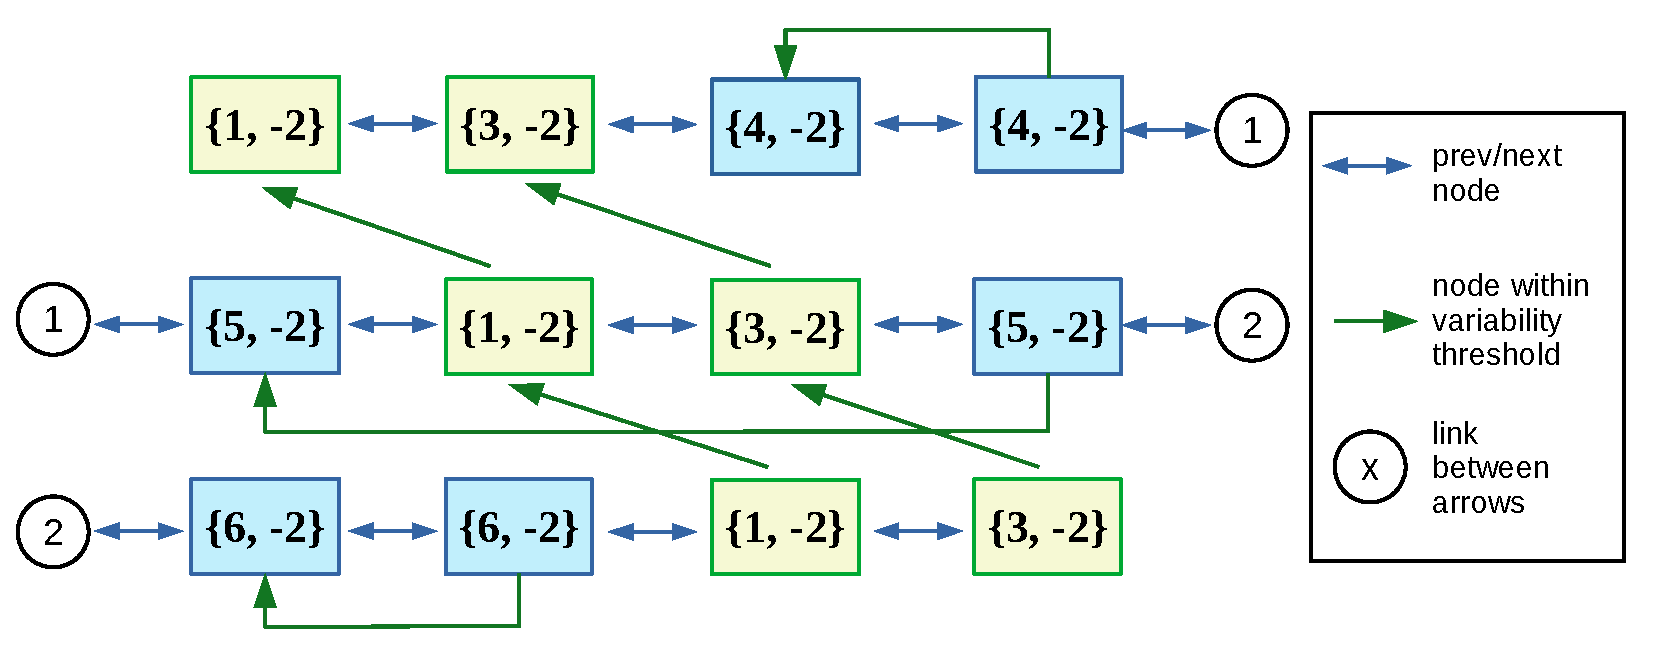
\includegraphics[width=1\columnwidth]{img/T2RGraph}
  \caption{Graph representation of the code example displayed in figure \ref{fig:2rvariabilityhigh4}.}
  \label{fig:clonerefactorprocess}
\end{figure}

In this graph, the duplicate relations (green arrows) do not necessarily denote an exact match. The duplicate relations allow for variability in the equality arrays as long as it falls under the variability threshold. However, negative numbers in the equality array may never vary. This is because negative numbers are the tokens/expressions that we do not allow variability in because they cannot be refactored as easily:
\begin{equation}\label{eq:t2rcloneequality}
E_1\text{ can only be cloned with }E_2\text{ iff }|E_1|=|E_2| \land \forall (x \in E_1, y \in E_2)\text{ }x<0 \lor y<0 \Rightarrow x=y
\end{equation}

\subsubsection{Detect Clones on Graph}
Similar to the clone detection process, we detect clones on basis of the graph described in the previous section. The only difference is that, in this step, we do not remove clones that do not meet the thresholds (as explained in section \ref{sec:clonerefactorthresholds}). This is because the next step, explained in the next section, could potentially expand the found clones and thus make clones that would currently invalid by the thresholds valid.

Looking back at the example of the previous section, it would result in the following clone class collection:
\begin{figure}[H]
\begin{parcolumns}{3}
\colchunk[1]{
\begin{javacode}
|\highlightYellow|doA(); // |\textcolor{pgreen}{$C_1$ $I_3$}|
|\highlightYellow|doB(); // |\textcolor{pgreen}{$C_1$ $I_3$}|
doC(); // |\textcolor{pgreen}{$C_4$ $I_2$}|
doC(); // |\textcolor{pgreen}{$C_4$ $I_1$}|
\end{javacode}}
\colchunk[2]{
\begin{javacode}
doD(); // |\textcolor{pgreen}{$C_3$ $I_2$}|
|\highlightYellow|doA(); // |\textcolor{pgreen}{$C_1$ $I_2$}|
|\highlightYellow|doB(); // |\textcolor{pgreen}{$C_1$ $I_2$}|
doD(); // |\textcolor{pgreen}{$C_3$ $I_1$}|
\end{javacode}}
\colchunk[3]{
\begin{javacode}
doE(); // |\textcolor{pgreen}{$C_2$ $I_2$}|
doE(); // |\textcolor{pgreen}{$C_2$ $I_1$}|
|\highlightYellow|doA(); // |\textcolor{pgreen}{$C_1$ $I_1$}|
|\highlightYellow|doB(); // |\textcolor{pgreen}{$C_1$ $I_1$}|
\end{javacode}}
\end{parcolumns}
\caption{Clone instances in figure \ref{fig:2rvariabilityhigh4} as determined .}
\label{fig:2rvariabilityhigh5}
\end{figure}

Where \textit{C} denotes the clone class and \textit{I} denotes the clone instance. The process by which these clones are found is equal to the clone detection process as described in section \ref{sec:detectingclones}. In this example, we see the four clones found on the graph of figure \ref{fig:clonerefactorprocess}. Three of these clone classes have a two clone instances, each consisting of a single nodes. The other clone class has three clone instances, each consisting of two nodes.

\subsubsection{Try to Expand}
The problem with the graph clone detection technique is that only single nodes that are within the variability threshold are considered duplicates of each other. However, single nodes that are not within this threshold could still be part of a clone class if the other cloned nodes are more towards the lower bound of the threshold.

\begin{figure}[H]
\begin{parcolumns}{2}
\colchunk[1]{
\begin{javacode}
|\highlightYellow|doA(a); //{1, -2, 7, -3, -4}
doB(a); //{5, -2, 7, -3, -4}
|\highlightYellow|doD(); //{8, -2, -3, -4}
|\highlightYellow|doE(); //{9, -2, -3, -4}
|\highlightYellow|doF(); //{10, -2, -3, -4}
doG(a); //{11, -2, 7, -3, -4}
\end{javacode}}
\colchunk[2]{
\begin{javacode}
|\highlightYellow|doA(a); //{1, -2, 7, -3, -4}
doC(a); //{6, -2, 7, -3, -4}
|\highlightYellow|doD(); //{8, -2, -3, -4}
|\highlightYellow|doE(); //{9, -2, -3, -4}
|\highlightYellow|doF(); //{10, -2, -3, -4}
doH(b); //{12, -2, 13, -3, -4}
\end{javacode}}
\end{parcolumns}
\caption{Type 2R clones with their equality arrays.}
\label{fig:trytoexpand}
\end{figure}

As an example, consider the clone fragment in figure \ref{fig:trytoexpand}. In this example, we have 2 clone classes. In the ``Try To Expand'' step, we will check whether we can create a clone class with larger clone instances on basis of the clones found in the previous step. We start with the largest clone class, measured in clone volume. We measure clone volume as the product of the amount of clone instances in a clone class and the amount of nodes in any of its instances.

In the example in figure \ref{fig:trytoexpand} the largest instance has a volume of:

\begin{equation}\label{eq:clonevolume}
3 \text{ nodes} * 2 \text{ clone instances} = 6
\end{equation}

Starting from this clone, we will try to expand it. We will include the previous node in the clone class and verify its variability threshold (node $N_2$). In this case, using the formulas shown in section \ref{sec:t2rcheckglobalthres}, we can check whether this clone class would be valid by the variability threshold:

\begin{equation}\label{eq:variabilitycombined1}
\frac{|\{(5,6)\}|}{|\{(5,6),(7,7),(8,8),(9,9),(10,10)\}|}*100 = \frac{1}{5}*100 = 20\%
\end{equation}

Dependent on the actual variability threshold, the clone class would get expanded with node $N_2$. For this example, we assume the variability threshold is set to 15\%. In such a case, including this node would not result in a valid clone class. However, we continue trying to expand this clone class until we have reached the first node of the originally cloned fragment (the cloned fragment that did not take the variability threshold into account). Thus, we now try to expand with $\{N_1, N_2\}$. We then get the following formula:

\begin{equation}\label{eq:variabilitycombined2}
\frac{|\{(5,6)\}|}{|\{(1,1),(7,7),(5,6),(7,7),(8,8),(9,9),(10,10)\}|}*100 = \frac{1}{7}*100 = 14\%
\end{equation}

This falls under the threshold of 15\% so we expand the clone class. Thus, the clone class $\{N_3, N_4, N_5\}$ will become $\{N_1, N_2, N_3, N_4, N_5\}$. We cannot expand further because we have reached the end of the original cloned fragment. When we are done expanding to previous nodes, we will try to expand to next nodes. In this case, we check whether we can include $N_6$ into the clone class. If $N_6$ would be included, the variability threshold would be as follows:

\begin{equation}\label{eq:variabilitycombined3}
\frac{|\{(5,6),(11,12),(7,13)\}|}{|\{(1,1),(7,7),(5,6),(7,7),(8,8),(9,9),(10,10),(11,12),(7,13)\}|}*100 = \frac{3}{9}*100 = 33\%
\end{equation}

This does not fall within the variability threshold, so we do not include this node in the clone class. After we have checked a single clone class within the bigger cloned fragment for expansion opportunities, we go on with the next clone class (by volume). In this case, the other clone class within this fragment has become a subset of the clone class we just expanded. Because of that, this other clone class is discarded. For the example code fragment in figure \ref{fig:trytoexpand} the resulting clone class is $\{N_1, N_2, N_3, N_4, N_5\}$.

\subsection{Checking for type 3 opportunities} \label{sec:t3rclonerefactor}
As described in section \ref{sec:type3r}, we define type 3R clones as gapped clones. This means that two existing clones may have a gap of non-gapped clones. We check for every found clone class whether it is a type 3R clone with another clone:

\begin{equation}\label{eq:crtype3r}
\forall (c_1 \in S) \text{ }\exists (c_2 \in S)\text{ }x \neq y \land isType3R(c_1, c_2)
\end{equation}

Where \textit{S} is the set of all found clone classes. $\text{isType3R}(C_1, C_2)$ is a Boolean-valued function that returns whether two clone classes are type 3R clones of each other. Two clone classes are type 3R clones of each other if each of their instances are within a certain distance of each other:

\begin{equation}\label{eq:istype3r}
\text{isType3R}(C_1, C_2) = \forall (i_1 \in C_1)\text{ } \exists (i_2 \in C_2)\text{ } Fi_1 = Fi_2 \land gap(i_1, i_2) < gap\_threshold
\end{equation}

Where \textit{F} is the file in which the clone instance is located. \textit{gap\_threshold} is the defined threshold percentage of the maximum gap size between two clone instances. $\text{gap}(I_1, I_2)$ is the function that calculates the gap between two clone instances. This gap is calculated by dividing the amount of statements in the gap by the amount of statements that both clone instances span together:

\begin{equation}\label{eq:t3rgap}
\text{gap}(i_1, i_2) = \frac{|\{(Rn>Ri_1 \land Rn<Ri_2) \lor (Rn>Ri_2 \land Rn<Ri_1)\text{ }|\text{ } n \in nodes(Fi_1)\}|}{|i_1| + |i_2|} * 100
\end{equation}

Where \textit{F} is the file in which the clone instance is located and \textit{R} is the range of a clone instance or node. A range denotes the line and column at which a code fragment starts and ends. We define the partial order relationship on ranges as follows:

\begin{equation}\label{eq:rangetotalorder}
r_1 < r_2 \text{ iff } ELr_1 < BLr_2 \lor (ELr_1 = BLr_2) \land ECr_1 < BCr_2)
\end{equation}
\begin{equation}\label{eq:rangetotalorder2}
r_1 > r_2 \text{ iff } BLr_1 > ELr_2 \lor (BLr_1 = ELr_2 \land BCr_1 > ECr_2)
\end{equation}

Where \textit{BL} is the begin line of a range, \textit{EL} is the end line of a range, \textit{BC} is the begin column of a range and \textit{EC} is the end column of a range.

\subsubsection{Example}
In this section we show an example of the identification of a type 3R clone.

\begin{figure}[H]
\begin{parcolumns}{2}
\colchunk[1]{
\begin{javacode}
//File1.java
|\highlightYellow|doA(); // |\textcolor{pgreen}{$C_1$ $I_1$}|
|\highlightYellow|doB(); // |\textcolor{pgreen}{$C_1$ $I_1$}|
doC();
|\highlightBlue|doC(); // |\textcolor{pgreen}{$C_2$ $I_1$}|
|\highlightBlue|doD(); // |\textcolor{pgreen}{$C_2$ $I_1$}|
\end{javacode}}
\colchunk[2]{
\begin{javacode}
//File2.java
|\highlightYellow|doA(); // |\textcolor{pgreen}{$C_1$ $I_2$}|
|\highlightYellow|doB(); // |\textcolor{pgreen}{$C_1$ $I_2$}|
|\highlightBlue|doC(); // |\textcolor{pgreen}{$C_2$ $I_2$}|
|\highlightBlue|doD(); // |\textcolor{pgreen}{$C_2$ $I_2$}|
\end{javacode}}
\end{parcolumns}
\caption{Gapped clones.}
\label{fig:3ropportunities}
\end{figure}

In the example of figure \ref{fig:3ropportunities} we see two clone classes, which are separated by a single node. Using equation \ref{eq:t3rgap} we can calculate the size of the gap as follows:

\begin{equation}\label{eq:t3rexample}
\text{gap}(C_1\text{ }I_1, C_2\text{ }I_1) = \frac{|\{n_4\}|}{|\{n_2, n_3\}| + |\{n_5, n_6\}|} * 100 = frac{1}{4} = 25\%
\end{equation}

The same calculation is conducted for the other clone instances:

\begin{equation}\label{eq:t3rexample}
\text{gap}(C_1\text{ }I_2, C_2\text{ }I_2) = \frac{|\emptyset|}{|\{n_2, n_3\}| + |\{n_4, n_5\}|} * 100 = frac{0}{4} = 0\%
\end{equation}

If all resulting percentages are under the threshold, this clone will be added to the collection of found clones and all of its subsets will be removed.

\section{Context Analysis of Clones}\label{chap:contextsetup}
To be able to refactor code clones, CloneRefactor first maps the context of code clones. We define the following aspects of the clone as its context:
\begin{enumerate}
  \item \textbf{Relation:} The relation of clone instances among each other through inheritance.
  \item \textbf{Location:} Where a clone instance occurs in the code.
  \item \textbf{Contents:} The statements/declarations of a clone instance.
\end{enumerate}
We define categories for each of these aspects and enable CloneRefactor to determine the catagories of clones.

\begin{figure}[H]
  \centering
    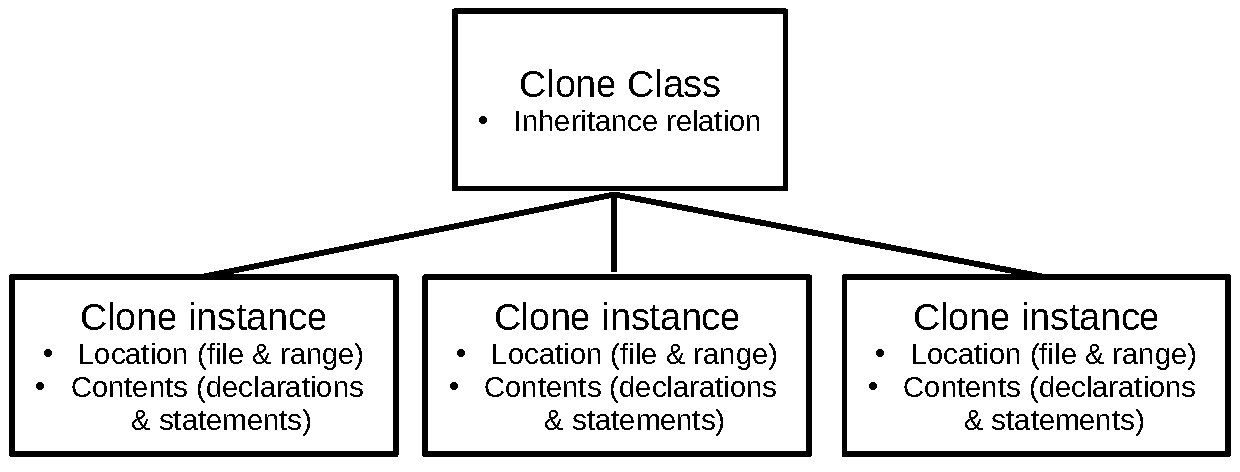
\includegraphics[width=0.8\columnwidth]{img/context}
    \caption{Abstract representation of clone classes and clone instances.}
  \label{fig:clonecontext}
\end{figure}

Fig.~\ref{fig:clonecontext} shows an abstract representation of clone classes and clone instances. The relation of clones through inheritance is measured for each clone class. The location and contents of clones are measured for each clone instance.

\subsection{Relation}\label{sec:setuprelation}
When merging code clones in object-oriented languages, it is important to consider the inheritance relation between clone instances. This relation has a big impact on how a clone should be refactored.

Fontana et al.~\cite{fontana2015duplicated} describe measurements on 50 open source projects on the relation of clone instances to each other. To do this, they first define several categories for the relation between clone instances in object-oriented languages. These categories are as follows:
\begin{enumerate}
  \item \textbf{Same Method}: All instances of the clone class are in the same method.
  \item \textbf{Same Class}: All instances of the clone class are in the same class.
  \item \textbf{Superclass}: All instances of the clone class are in a class that is child or parent of each other.
  \item \textbf{Sibling Class}: All instances of the clone class have the same parent class.
    \item \textbf{Ancestor Class}: All instances of the clone class are superclasses except for the direct superclass.
  \item \textbf{First Cousin Class}: All instances of the clone class have the same grandparent class.
\item \textbf{Same Hierarchy Class}: All instances of the clone class belong to the same inheritance hierarchy, but do not belong to any of the other categories.
\item \textbf{Same External Superclass}: All instances of the clone class have the same superclass, but this superclass is not included in the project but part of a library.
\item \textbf{Unrelated class}: There is at least one instance in the clone class that is not in the same hierarchy.
\end{enumerate}

We added the following categories, to gain more information about clones and reduce the number of unrelated clones:

\begin{enumerate}
\item \textbf{Same Interface}: All instances of the clone class are in a class or interface that have a common interface anywhere in their inheritance hierarchy.
\item \textbf{No Direct Superclass}: All instances of the clone class are in a class that does not have any superclass.
\item \textbf{No Indirect Superclass}: All instances of the clone class are in a class that does not have any external classes in its inheritance hierarchy.
\item \textbf{External Ancestor}: All instances of the clone class are in a class that does not have any external classes in its inheritance hierarchy.
\end{enumerate}

Figure \ref{fig:clonecontext} shows an abstract representation of clone classes and clone instances. The relation of clones through inheritance is measured on clone class level: it involves all child clone instances. The location and contents of clones is measured on clone instance level. A clone's location involves the file it resides in and the range it spans (for example: line 6 col 2 - line 7 col 50). A clone instance contents consists of a list of all statements and declarations it spans.

\begin{figure}[H]
  \centering
    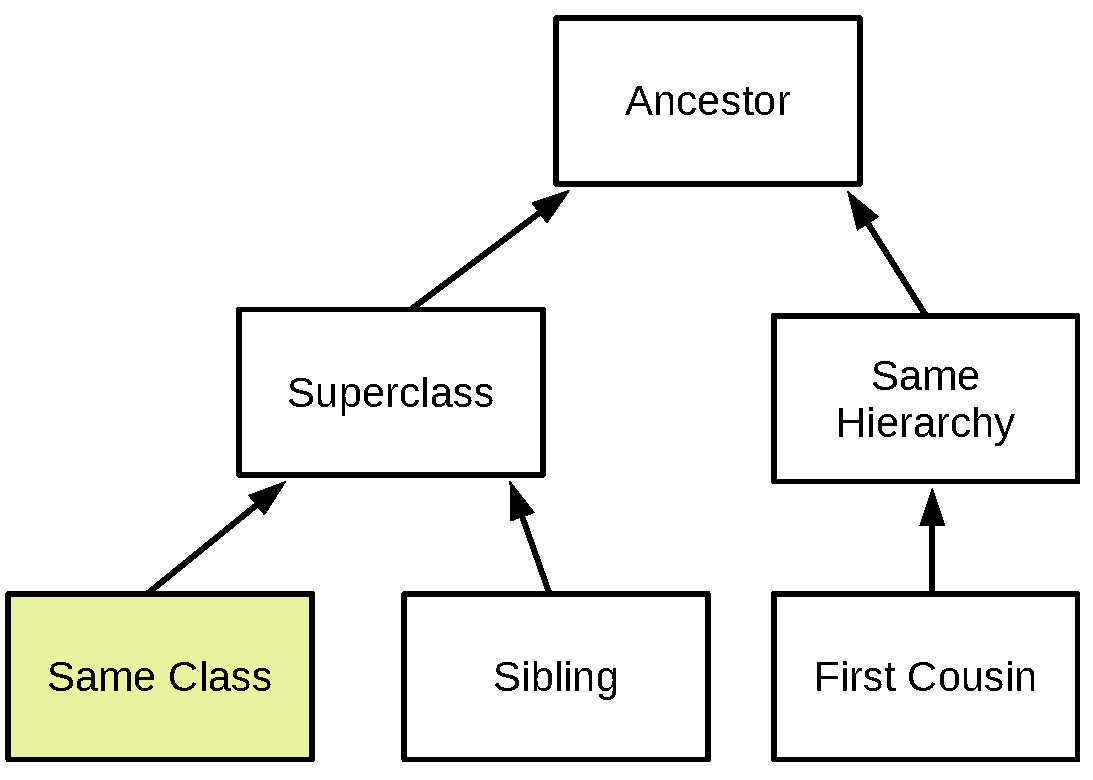
\includegraphics[width=0.6\columnwidth]{img/Relation}
      \caption{Abstract figure displaying relations of clone classes. Arrows represent superclass relations.}
  \label{fig:clonerelation}
\end{figure}

We separate these relations into the following categories, because of their related refactoring opportunities:
\begin{itemize}
  \item \textbf{Common Class}: \textit{Same Method}, \textit{Same Class}
  \item \textbf{Common Hierarchy}: \textit{Superclass}, \textit{Sibling Class}, \textit{Ancestor Class}, \textit{First Cousin}, \textit{Same Hierarchy}
  \item \textbf{Common Interface}: \textit{Same Interface}
  \item \textbf{Unrelated}: \textit{No Direct Superclass}, \textit{No Indirect Superclass}, \textit{External Superclass}, \textit{External Ancestor}
\end{itemize}

Every clone class only has a single relation, which is the first relation from above list that the clone class applies to. For instance: all ``Superclass'' clones also apply to ``Same Hierarchy'', but because ``Superclass'' is earlier in above list they will get the ``Superclass'' relation. This is because the items earlier in the list denote a more favorable refactoring.

To check a the relation for a given clone class, we compare each node in a clone instance with the respective nodes in each other clone instance within a clone class. So for a clone class with x clone instances and each clone instance has y nodes, we perform:

\begin{equation}\label{eq:sameclass}
\frac{x * (x + 1)}{2} * y
\end{equation}

comparisons to determine the relation. Each of these checks will result in one of the relations from the list above. Of these relations, the item lowest in the list is going to be the relation of the clone class. So for instance, if a clone class has 15 nodes that denote a \textit{Superclass} relation but 3 nodes are \textit{Unrelated}, the clone class becomes \textit{Unrelated}.

\subsubsection{Common Class}
The \textit{Same method} and \textit{Same class} relations share a common refactoring opportunity. Clones of both these catagories, when extracted to a new method, can be placed in the same class. Both of these relations are most favorable for refactoring, as they require a minimal design tradeoff. Furthermore, global variables that are used in the class can be used without having to create method parameters.

Cloned nodes are flagged as \textit{Same method} if these nodes are found in the same method. We define the method as the first method declaration that is encountered when following the parent nodes in the ast for a given cloned node. Please note that a clone instance may not always be in a method, for which this predicate will fail.

Cloned nodes are flagged as \textit{Same class} if these nodes are found in the same class. We define the class as the first class declaration that is encountered when following the parent nodes in the ast for a given cloned node.

\subsubsection{Common Hierarchy}
Clones that are in a common hierarchy can be refactored by using the ``Extract Method'' refactoring method followed by ``Pull Up Method'' until the method reaches a location that is accessible by all clone instances. However, the more often ``Pull Up Method'' has to be used, the more detrimental the effect is on system design. This is because putting a lot of functionality in classes higher up in an inheritance structure can result in the ``God Object'' anti-pattern. A god object is an object that knows too much or does too much.

Cloned nodes are flagged as \textit{Superclass} if the classes in which these nodes are found are parent and child class of each other. Cloned nodes are flagged as \textit{Siblings} if the classes in which these nodes are found all share the same parent and this parent class is not external. Cloned nodes are flagged as \textit{First Cousin} if the classes in which these nodes are found all share the same grandparent and this grandparent class is not external.

Cloned nodes are flagged as \textit{Ancestor} if the classes in which these nodes are found are recursively the parent of an antecedent. Cloned nodes are flagged as \textit{Same Hierarchy} if the classes in which these nodes are found are all in the same inheritance hierarchy and not linked by any external classes.

\subsubsection{Common Interface}
Many object-oriented languages know the concept of ``interfaces'', which are used to specify a behavior that classes must implement. As code clones describe functionality and interfaces originally did not allow for functionality, interfaces did not open up refactoring opportunities for duplicated code. However, many programming languages nowadays support default implementations in interfaces. Since Java 7 and C\#8, these programming languages allow for functionality to be defined in interfaces. Many other object-oriented languages like Python allow this by nature, as they do not have a true notion of interfaces.

The greatest downside on system design of putting functionality in interfaces is that interfaces are per definition part of a classes' public contract. That is, all functionality that is shared between classes via an interface cannot be hidden by setting a stricter visibility. Because of that, we favor all ``Common Hierarchy'' refactoring opportunities over ``Common Interface''.

To check whether two cloned nodes have common interfaces, we recursively walk all types the class or interface of the cloned nodes implement and extend. The common interface that is closest to the cloned node in terms of depth of recursion will be flagged as the refactoring candidate.

\subsubsection{Unrelated}
Clones are unrelated if they share no common class or interface in their inheritance structure. These clones are least favorable when looking at refactoring, because their refactoring will almost always have a major impact on system design. We formulated four catagories of unrelated clones to look into their refactoring opportunities.

Cloned nodes are flagged \textit{No Direct Superclass} if they are in classes that do currently not have a parent. This marks the opportunity for creating a superclass abstraction and placing the extracted method there. Cloned nodes are flagged \textit{No Indirect Superclass} if any of their ancestors does not have a parent. In such a case, it would be possible to create such an abstraction for the ancestor that does not have a parent.

Cloned nodes are flagged \textit{External Superclass} if they are in a class which has an external parent. Cloned nodes are flagged \textit{External Ancestor} if one of their ancestors has an external parent. Both of these relations obstruct the possibility of creating a superclass abstraction. In such a case, an interface abstraction could be created to make their relation explicit.

\subsection{Location}\label{sec:setuplocation}
A paper by Lozano et al. \cite{lozano2007evaluating} discusses the harmfulness of cloning. The authors argue that 98\% are produced at method-level. However, this claim is based on a small dataset and based on human copy-paste behavior rather than static code analysis. We decided to measure the locations of clones through static analysis on our dataset. We chose the following categories:
\begin{enumerate}
  \item \textbf{Method/Constructor Level:} A clone instance that does not exceed the boundaries of a single method or constructor (optionally including the declaration of the method or constructor itself).
  \item \textbf{Class Level:} A clone instance in a class, that exceeds the boundaries of a single method or contains something else in the class (like field declarations, other methods, etc.).
  \item \textbf{Interface Level:} A clone that is (a part of) an interface.
  \item \textbf{Enumeration Level:} A clone that is (a part of) an enumeration.
\end{enumerate}
We check the location of each clone instance for each of its nodes. If any node reports a different location from the others, we choose the location that is lowest in above list. So for instance, if a clone instance has 15 nodes that denote a \textit{Method Level} location but 3 nodes are \textit{Class Level}, the clone instance becomes \textit{Class Level}.

\todo{Explain why these categories indicate and how they are related to refactoring}

\subsection{Contents}\label{sec:setupcontents}
Finally, we looked at what nodes individual clone instances span. We selected the following categories to be relevant for refactoring:
\begin{enumerate}
  \item \textbf{Full Method/Class/Interface/Enumeration:} A clone that spans a full class, method, constructor, interface or enumeration, including its declaration.
  \item \textbf{Partial Method/Constructor:} A clone that spans a method partially, optionally including its declaration.
  \item \textbf{Several Methods:} A clone that spans over two or more methods, either fully or partially, but does not span anything but methods (so not fields or anything in between).
  \item \textbf{Only Fields:} A clone that spans only global variables.
  \item \textbf{Includes Fields/Constructor:} A clone that spans a combination of fields and other things, like methods.
  \item \textbf{Method/Class/Interface/Enumeration Declaration:} A clone that contains the declaration (usually the first line) of a class, method, interface or enumeration.
  \item \textbf{Other:} Anything that does not match with above-stated categories.
\end{enumerate}

\todo{Explain each category in more detail}

\section{Method extraction opportunities}\label{sec:refactorabilitysetup}
The most used technique to refactor clones is method extraction (creating a new method on basis of the contents of clones). However, method extraction cannot be applied in all cases. In these instances, more conditions may apply to be able to conduct a refactoring, if beneficial at all.

We measured the number of clones that can be refactored through method extraction (without additional transformations being required). We defined the following categories:
\begin{itemize}
    \item \textbf{Can be extracted:} This clone is a fragment of code that can directly be extracted to a method. Then, based on the relation between the clone instances, further refactoring techniques can be used to refactor the extracted methods (for instance ``pull up method'' for clones in sibling classes).
    \item \textbf{Complex control flow:} This clone contains \texttt{break}, \texttt{continue} or \texttt{return} statements, obstructing the possibility of method extraction.
    \item \textbf{Spans part of a block:} This clone spans a part of a statement.
    \item \textbf{Is not a partial method:} If the clone does not fall in the ``Partial method'' category of Table~\ref{table:contents}, the ``extract method'' refactoring technique cannot be applied.
\end{itemize}

\todo{Explain each category in more detail}
